\section{Question1}
\begin{enumerate}[a).]
\item  \textbf{algorithm description:} \\	
Let ``query($X,k$)'' denotes the $k^{th}$ smallest number of $A$ or $B$ and 
we call two databases $A=\{a_1,a_2,...,a_i,...,a_n\},B=\{b_1,b_2,...,b_j,...,b_n\}$ arranged in
ascending order
(In fact,it does no matter to care the sequence order owing to ``query''  ).\\
$\text{query}(A,i)$ can be written as $a_i$,as well as $\text{query}(B,j)$.
Making sure $i+j=n$ , 
\begin{itemize}
	\item  if $a_i < b_j$, the median lies in $\{a_{i+1},...,a_n\} \bigcup \{b_1,b_2,...,b_j\}$;
	\item  if $a_i = b_j$, the median is $a_i$ or $b_j$;
	\item  if $a_i > b_j$, the median lies in $\{a_1,a_2,...,a_i\} \bigcup \{b_{j+1},...,b_n \}$
\end{itemize}
We initialize $i = n/2, j = n -i$,that equals to comparing the median of each database.
Then the search area can be narrowed down to half length of the last
until we just need to find $1^{th}$ smallest number between two separate arrays. \\
pseudo-code:
\begin{algorithm}[H]
\caption{finding the median of two separate databases via query}
\begin{algorithmic}[1]
\Require Two separate databases $A$,$B$,length $n$. (initializing $i,j=0,k=n$)	
\Ensure  the median(the $n^{th}$ smallest) of $A\bigcup B$
\Function {find\_kth}{$A,i,B,j,k$}
\If {$k = 1$}
\State \Return $\min \{\text{query}(A,i+1),\text{query}(B,j+1)
		\} $
\EndIf
\If {$i = 0$ (initial)}
\State $i \gets k/2, j \gets k - i$
\EndIf
\If {$\text{query}(A,i) < \text{query}(B,j)$}
\State $ k \gets k - k/2$ (each discards $k/2$ numbers)
\State $ i \gets i + k/2, j \gets j - k/2$
\If {$k=1$}
\State $j \gets j-1$
\EndIf

\State \Return \Call{find\_kth}{$A,i,B,j,k$}
\ElsIf {$\text{query}(A,i) > \text{query}(B,j)$}
\State $k \gets k-k/2,i \gets i - k/2,j \gets j + k/2$
\If {$k=1$}
\State $i \gets i-1$
\EndIf
\State \Return \Call{find\_kth}{$A,i,B,j,k$}
\Else
\State \Return $\text{query}(A,i)$
\EndIf
\EndFunction
\end{algorithmic}	
\end{algorithm}

\item \textbf{subproblem reduction graph}
\begin{figure}[H]
\centering
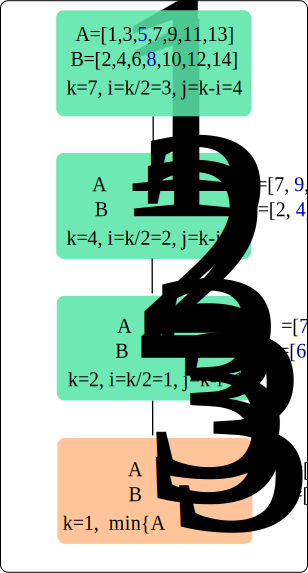
\includegraphics[width=0.45\textwidth,height=0.4\textheight]{pictures/graph_median}	
\caption{problem instance}
\end{figure}
\item \textbf{proof of the correctness} \\
%it may be difficult...
Obviously, $k = 1$ means that we just want the $1^{th}$ smallest number of
$A\bigcup B$.
In order to find the median of $A\bigcup B$,we initialize $i = n/2, j= n-i, k = n$.
Let ``$A[i]$'' denotes ``$\text{query}(A,i)$'',
then compare $A[i]$ with $B[j]$: 
\begin{enumerate}[i.]
	\item   if $A[i] < B[j]$, we can surely say that $\{A[1],A[2],...,A[i]\}$ must lies in the left of 
		  the median and $\{B[j+1],...,B[n]\}$ must lies in the right of the median.For instance,
		  if $B[j+1]$ is the median,then there has $i+j=n$ numbers smaller than $B[j+1]$
		   (each element of $\{A[1],...,A[i]\}\cup \{B[1],B[2],...,B[j]\}$ is smaller than $B[j+1]$
		   ).
	\item if $A[i] = B[j]$, the median is $A[i]$ (or $B[j]$).
	\item if $A[i] > B[j]$,it's the opposite of i. 	   		   
\end{enumerate}
in each iteration, we discard $k/2$ numbers until $k=1$.	

\item \textbf{complexity of the algorithm}  \\
The size of original problem is reduced to half at each iteration,
and ``query'' costs $O(1)$,thus \\
\[
T(n) = T(n/2) + cO(1) = O(\log n)
\]
	
\end{enumerate}